% LaTeX Template for short student reports.
% Citations should be in bibtex format and go in references.bib
\documentclass[a4paper, 11pt]{article}
\usepackage[top=3cm, bottom=3cm, left = 2cm, right = 2cm]{geometry} 
\geometry{a4paper} 
\usepackage[utf8]{inputenc}
\usepackage{textcomp}
\usepackage{graphicx} 
\usepackage{amsmath,amssymb}  
\usepackage{bm} 
\usepackage{tikz}
\usepackage[pdftex,bookmarks,colorlinks,breaklinks]{hyperref}  
%\hypersetup{linkcolor=black,citecolor=black,filecolor=black,urlcolor=black} % black links, for printed output
\usepackage{memhfixc} 
\usepackage{pdfsync}  
\usepackage{fancyhdr}
\pagestyle{fancy}

\title{Perbandingan Kinerja Metode Verifikasi Wajah Menggunakan Library DeepFace pada Dataset FaceScrub}
\author{Najwan Yusnianda\\NIM: 2408207010029}
\date{}

\begin{document}

\maketitle



\section{Pendahuluan}

Teknologi pengenalan dan verifikasi wajah telah mengalami perkembangan signifikan dalam beberapa tahun terakhir, seiring dengan kemajuan di bidang deep learning, khususnya dalam domain Visi Komputer. Proses verifikasi wajah, yaitu memastikan bahwa dua gambar wajah berasal dari individu yang sama, menjadi semakin penting dalam berbagai aplikasi praktis, seperti sistem keamanan perbankan, pemasaran digital, hiburan, dan layanan publik.

Namun, kinerja metode verifikasi wajah sangat bergantung pada model yang digunakan, parameter yang diterapkan, serta kualitas dataset yang digunakan untuk melatih model. Penelitian ini bertujuan untuk membandingkan kinerja beberapa model verifikasi wajah yang tersedia dalam library DeepFace, sebuah framework deep learning yang dirancang khusus untuk tugas-tugas pengenalan wajah. Penelitian dilakukan menggunakan dataset FaceScrub , yang mencakup gambar wajah publik figur dengan variasi pose, pencahayaan, dan ekspresi.

Tujuan utama dari penelitian ini adalah untuk mengevaluasi efektivitas model seperti Facenet512 , Facenet , dan VGG-Face dalam melakukan verifikasi wajah menggunakan dataset FaceScrub. Hasil dari penelitian ini diharapkan dapat memberikan wawasan tentang performa masing-masing model , sehingga dapat membantu pengembang dan peneliti dalam memilih model yang paling sesuai untuk aplikasi terutama dalam verifikasi wajah indvidu yang sama.


\section{Metodologi}
Penelitian ini dirancang untuk membandingkan kinerja beberapa model verifikasi wajah yang tersedia dalam library DeepFace menggunakan dataset FaceScrub . Gambar wajah diproses melalui serangkaian tahapan, mulai dari pengumpulan data hingga evaluasi model.

\begin{figure}[h]
    \centering
    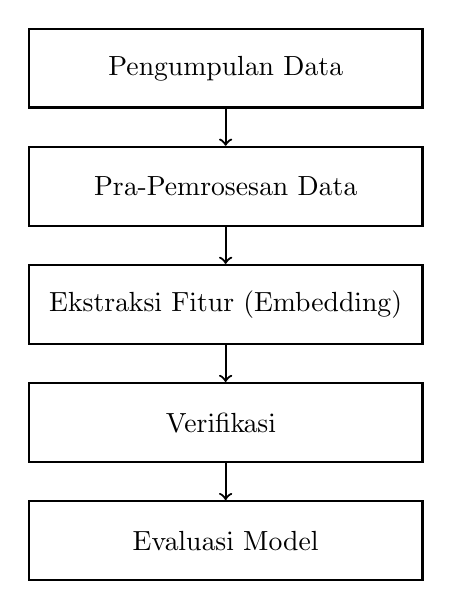
\begin{tikzpicture}[
        node distance=1.5cm,
        every node/.style={draw, rectangle, minimum width=5cm, minimum height=1cm, align=center},
        every path/.style={draw, ->, thick}
    ]
        % Nodes
        \node (data) {Pengumpulan Data};
        \node (preprocess) [below of=data] {Pra-Pemrosesan Data};
        \node (embedding) [below of=preprocess] {Ekstraksi Fitur (Embedding)};
        \node (verification) [below of=embedding] {Verifikasi };
        \node (evaluation) [below of=verification] {Evaluasi Model};

        % Arrows
        \path (data) -- (preprocess);
        \path (preprocess) -- (embedding);
        \path (embedding) -- (verification);
        \path (verification) -- (evaluation);
    \end{tikzpicture}
    \caption{Flowchart tahapan penelitian}
    \label{fig:flowchart}
\end{figure}



\subsection{Pengumpulan Dataset}


Dataset yang digunakan dalam penelitian ini adalah FaceScrub , yang mencakup gambar wajah dari berbagai aktor dan aktris yang bervariasi.Dataset terdiri dari 200 aktor/aktris yang dipilih secara acak dari keseluruhan dataset 
Dataset dibagi menjadi dua subset: sampel set dan testing set.setiapa aktor/aktris yang sama, masing-masing memiliki 20 gambar sebagai sampel dan 5 gambar untuk testing untuk memastikan evaluasi yang adil dan objektif

\subsection{Deteksi Wajah}

Deteksi wajah pada merupakan langkah awal yang sangat penting dalam  verifikasi wajah dalam dataset facescrub. Pada penelitian ini, deteksi wajah dilakukan menggunakan framework \textbf{MTCNN} (Multi-task Cascaded Convolutional Networks). MTCNN adalah salah satu metode deteksi wajah yang terkenal karena kemampuannya mendeteksi wajah dengan akurasi tinggi meskipun dalam kondisi variasi pose, pencahayaan, atau resolusi rendah.

Setelah wajah terdeteksi, area wajah tersebut dipotong menjadi \textit{Region of Interest} (RoI) untuk memastikan bahwa proses verifikasi hanya berfokus pada fitur-fitur wajah yang relevan. Proses ini membantu mengurangi noise dari latar belakang gambar dan meningkatkan akurasi model dalam mengenali wajah.

Aturan yang digunakan dalam tahap ini adalah sebagai berikut:

\begin{enumerate}
    \item Jika wajah berhasil terdeteksi oleh MTCNN, maka area wajah (\textit{RoI}) akan diekstraksi dan dimasukkan kedalam dataset final yang digunakan untuk proses verifikasi.
    \item Jika wajah tidak terdeteksi (misalnya, karena kualitas gambar buruk atau wajah tidak tampak jelas), gambar tersebut diabaikan dan tidak digunakan dalam verifikasi.
\end{enumerate}

Pemilihan MTCNN sebagai alat deteksi wajah didasarkan pada kemampuannya untuk menghasilkan hasil yang bagus dan efisien.


\subsection{Verifikasi Wajah Menggunakan DeepFace}
Untuk setiap pasangan gambar wajah dalam dataset, model DeepFace digunakan untuk menghitung skor kesamaan (similarity score ) antara dua gambar.
Metode verifikasi yang diterapkan berdasarkan ambang batas (threshold ) yang ditentukan yaitu 0.4 dan 0.5 dengan cosine measure Jika skor kesamaan melebihi ambang batas, maka kedua gambar dianggap berasal dari individu yang sama.

Metode verifikasi wajah dibangun dengan membandingkan pasangan wajah dari set pengujian menggunakan fungsi verifikasi dari DeepFace yaitu :Facenet,Facenet512, dan VGG-Face.

\subsection{Evaluasi Kinerja}

Untuk mengukur kinerja dari model yang dievaluasi digunakan metrik penilaian sebagai berikut:
\begin{itemize}
    \item \textbf{True Positives (TP)}: Jumlah pasangan wajah yang benar-benar cocok.
    \item \textbf{False Positives (FP)}: Jumlah pasangan wajah yang salah cocok.
    \item \textbf{False Negatives (FN)}: Jumlah pasangan wajah yang salah tidak cocok.
    \item \textbf{True Negatives (TN)}: Jumlah pasangan wajah yang benar-benar tidak cocok.
    \item \textbf{Precision}: Rasio prediksi positif yang benar.
    \item \textbf{Recall}: Rasio prediksi positif yang benar terhadap jumlah positif yang sebenarnya.
    \item \textbf{F1-score}: Rata-rata harmonis dari Precision dan Recall.
\end{itemize}

Nilai F1-score digunakan sebagai indikator utama untuk menilai kinerja dari metode yang ditentukan.

\[
\text{F1-score} = 2 \times \frac{\text{Precision} \times \text{Recall}}{\text{Precision} + \text{Recall}}
\]

\section{Hasil dan Diskusi}




\subsection{Proses Embedding Gambar}

Dalam melakukan verifikasi wajah, setiap gambar wajah perlu dikonversi menjadi representasi numerik (embedding) sebelum dibandingkan. Proses ini dilakukan dengan mengekstrak fitur dari setiap wajah menggunakan model deep learning yang telah dilatih sebelumnya. Model yang digunakan dalam eksperimen ini adalah Facenet512 , Facenet , dan VGG-Face , yang masing-masing memiliki arsitektur Neural NetwoRk dalam untuk menghasilkan embedding yang merepresentasikan ciri-ciri unik dari wajah dalam bentuk vektor berdimensi tinggi.

Setiap gambar wajah \( x \) diproses melalui model deep learning \( f(x) \) untuk menghasilkan vektor embedding \( E \) dengan dimensi tertentu:

\begin{equation}
E = f(x)
\end{equation}

dimana:
\begin{itemize}
    \item \textbf{Facenet512} menghasilkan embedding berdimensi \textbf{512}.
    \item \textbf{Facenet} menghasilkan embedding berdimensi \textbf{128}.
    \item \textbf{VGG-Face} menghasilkan embedding berdimensi \textbf{4096}.
\end{itemize}

Proses embedding ini bertujuan untuk mentransformasikan data citra wajah ke dalam ruang fitur di mana wajah yang mirip akan memiliki representasi yang lebih dekat satu sama lain dalam metrik tertentu, seperti \textit{Euclidean Distance} atau \textit{Cosine Similarity}. 

Setelah proses deteksi wajah menggunakan MTCNN, setiap wajah yang berhasil terdeteksi diekstraksi dan direpresentasikan dalam bentuk vektor embedding. Embedding ini dihasilkan menggunakan tiga model berbeda, yaitu VGG-Face, FaceNet, dan FaceNet dengan dimensi 512.

Tabel \ref{tab:embedding_files} menunjukkan daftar file embedding yang digunakan dalam penelitian ini beserta ukuran file masing-masing. File embedding ini dibagi menjadi dua bagian utama: \textit{train embeddings} untuk data latih dan \textit{test embeddings} untuk data uji.

\begin{table}[h]
    \centering
    
    \begin{tabular}{|l|r|}
        \hline
        \textbf{Nama File Embedding} & \textbf{Ukuran File (KB)} \\
        \hline
        embedding\_VGG-Face\_train\_embeddings.pkl & 125.654 \\
        embedding\_VGG-Face\_test\_embeddings.pkl  & 31.433 \\
        embedding\_Facenet\_train\_embeddings.pkl  & 4.176 \\
        embedding\_Facenet\_test\_embeddings.pkl   & 1.048 \\
        embedding\_Facenet512\_train\_embeddings.pkl & 15.935 \\
        embedding\_Facenet512\_test\_embeddings.pkl  & 3.989 \\
        \hline
    \end{tabular}
    \caption{Daftar file hasil embedding berdasrkan model dan Ukurannya}
    \label{tab:embedding_files}
\end{table}

Dari tabel \ref{tab:embedding_files}, dapat dilihat bahwa embedding yang dihasilkan oleh model VGG-Face memiliki ukuran yang jauh lebih besar dibandingkan dengan model FaceNet dan FaceNet512. Hal ini disebabkan oleh kompleksitas arsitektur VGG-Face yang menghasilkan dimensi embedding yang lebih tinggi. Sebaliknya, model FaceNet dan FaceNet512 menghasilkan embedding dengan ukuran yang lebih kecil, yang dapat mengurangi kebutuhan penyimpanan dan mempercepat proses verifikasi.



\subsection{Eksperimen Verifikasi Wajah}
Evaluasi kinerja model dalam tugas verifikasi wajah dengan individu yang sama dilakukan dengan menggunakan dataset yang terdiri dari pasangan gambar wajah pada sampel dan pengujian (testing). Gambar wajah dalam set sampel dibandingkan dengan gambar dalam set pengujian menggunakan model DeepFace, yaitu Facenet512, Facenet, dan VGG-Face dengan threshold 0.4 dan 0.5.

Tabel \ref{tab:face_verification} menunjukkan beberapa contoh hasil eksperimen verifikasi wajah yang dilakukan menggunakan model Facenet512. Kolom Train Image dan Test Image menunjukkan pasangan gambar yang dibandingkan, sementara kolom Verified menampilkan label kebenaran (ground truth) dari pasangan tersebut. Kolom $y_{true}$ merepresentasikan label asli dari pasangan wajah, sedangkan $y_{pred}$ menunjukkan prediksi yang diberikan oleh model. Kolom Distance menunjukkan jarak antara dua gambar berdasarkan fitur yang diekstrak oleh model. Semakin kecil nilai jarak (Distance), semakin mirip kedua gambar tersebut.
\begin{table}[h]
    \centering
    \begin{tabular}{|c|c|c|c|c|c|c|}
        \hline
        Train Image & Test Image & Verified & $y_{true}$ & $y_{pred}$ & Distance & Model \\
        \hline
        Aaron\_Eckhart\_11\_11.jpeg & Aaron\_Eckhart\_108\_84.jpeg & True & 1 & 1 & 0.245835 & Facenet512 \\
        Aaron\_Eckhart\_149\_109.jpeg & Aaron\_Eckhart\_108\_84.jpeg & True & 1 & 1 & 0.456095 & Facenet512 \\
        Aaron\_Eckhart\_187\_132.jpeg & Aaron\_Eckhart\_108\_84.jpeg & True & 1 & 1 & 0.241423 & Facenet512 \\
        Aaron\_Eckhart\_188\_133.jpeg & Aaron\_Eckhart\_108\_84.jpeg & True & 1 & 1 & 0.442150 & Facenet512 \\
        Aaron\_Eckhart\_196\_140.jpeg & Aaron\_Eckhart\_108\_84.jpeg & True & 1 & 1 & 0.295349 & Facenet512 \\
        \hline
    \end{tabular}
    \caption{Contoh hasil eksperimen verifikasi wajah yang dilakukan}
    \label{tab:face_verification}
\end{table}

Dari hasil pada tabel \ref{tab:face_verification}, terlihat bahwa semua pasangan gambar yang diuji berhasil diverifikasi dengan benar oleh model Facenet512. Selain itu, nilai Distance yang rendah menunjukkan bahwa model berhasil mengidentifikasi kemiripan antara gambar wajah dalam pasangan yang diuji pada orang yang sama.

\subsection{Hasil Verifikasi Wajah}

Tabel \ref{tab:face_models_04} dan  \ref{tab:face_models_05} menunjukkan hasil evaluasi kinerja model verifikasi wajah menggunakan metrik yang telah disebutkan sebelumnya, dengan dua nilai ambang batas (threshold), yaitu 0.4 dan 0.5.

\begin{table}[h]
    \centering
    \begin{tabular}{|c|c|c|c|c|c|c|c|c|}
        \hline
        Model & TP & TN & FP & FN & Accuracy & Precision & Recall & F1-Score \\
        \hline
        Facenet512 & 11881 & 0 & 0 & 7709 & 0.606483 & 1.0 & 0.606483 & 0.755044 \\
        Facenet & 11910 & 0 & 0 & 7680 & 0.607963 & 1.0 & 0.607963 & 0.756190 \\
        VGG-Face & 3229 & 0 & 0 & 16361 & 0.164829 & 1.0 & 0.164829 & 0.283010 \\
        \hline
    \end{tabular}
    \caption{Perbandingan Kinerja Model Verifikasi Wajah dengan Threshold 0.4}
    \label{tab:face_models_04}
\end{table}

Dari hasil yang ditampilkan pada tabel \ref{tab:face_models_04} , terlihat bahwa model Facenet512 dan Facenet memiliki kinerja yang relatif serupa pada threshold 0.4, dengan  F1-score di kisaran 0.75. Sementara itu, model VGG-Face menunjukkan performa yang jauh lebih rendah, dengan F1-score sebesar 0.283. Hal ini menunjukkan bahwa VGG-Face kurang efektif dalam melakukan verifikasi wajah dibandingkan dengan Facenet512 dan Facenet pada dataset facescrub.

Pada tabel \ref{tab:face_models_05}, ambang batas diubah menjadi 0.5 sehingga menghasilkan peningkatan yang cukup signifkan pada nilai F1-score untuk semua model. Model Facenet512 mendapat nilai  F1-score 0.88, yang merupakan nilai tertinggi dibandingkan dengan model lainnya. Model Facenet memiliki kinerja yang sedikit lebih rendah dengan  F1-score 0.87. Sementara itu, meskipun VGG-Face mengalami peningkatan kinerja dibandingkan dengan threshold 0.4, hasilnya masih jauh lebih rendah daripada model Facenet, dengan dan F1-score 0.507.




\begin{table}[h]
    \centering
    \begin{tabular}{|c|c|c|c|c|c|c|c|c|}
        \hline
        Model & TP & TN & FP & FN & Accuracy & Precision & Recall & F1-Score \\
        \hline
        Facenet512 & 15414 & 0 & 0 & 4176 & 0.786830 & 1.0 & 0.786830 & 0.880699 \\
        Facenet & 15208 & 0 & 0 & 4382 & 0.776314 & 1.0 & 0.776314 & 0.874073 \\
        VGG-Face & 6657 & 0 & 0 & 12933 & 0.339816 & 1.0 & 0.339816 & 0.507258 \\
        \hline
    \end{tabular}
    \caption{Perbandingan Kinerja Model Verifikasi Wajah dengan Threshold 0.5}
    \label{tab:face_models_05}
\end{table}

Dari hasil ini, dapat disimpulkan bahwa dalam mengidentifikasi wajah dengan dataset Facescrub, Model Facenet512 menunjukkan kinerja terbaik dalam tugas verifikasi wajah, diikuti oleh Facenet, sedangkan VGG-Face memiliki kinerja yang paling rendah.
Kinerja  model VGG-Face dapat disebabkan oleh beberapa faktor. Salah satu faktor utama adalah dimensi embedding yang lebih tinggi dibandingkan dengan model lainnya, yang dapat menyebabkan overfitting dan menurunkan kemampuan model dalam melakukan generalisasi pada data uji.

Secara keseluruhan, model Facenet512 menunjukkan hasil terbaik antara ukuran embedding, efisiensi komputasi, dan akurasi dalam tugas verifikasi wajah pada dataset FaceScrub. 




\section{Kesimpulan}
Penelitian ini membandingkan kinerja beberapa model verifikasi wajah, yaitu Facenet512, Facenet, dan VGG-Face, menggunakan library DeepFace pada dataset FaceScrub. Hasil eksperimen menunjukkan bahwa Facenet512 memiliki performa terbaik dalam tugas verifikasi wajah, diikuti oleh Facenet yang menawarkan keseimbangan antara akurasi dan efisiensi komputasi. Sebaliknya, VGG-Face menunjukkan performa yang lebih rendah, kemungkinan disebabkan oleh dimensi embedding yang sangat besar, yang mengarah pada overfitting dan kesulitan dalam generalisasi.

Penelitian ini menegaskan bahwa pemilihan model verifikasi wajah harus mempertimbangkan keseimbangan antara akurasi, efisiensi komputasi, dan kemampuan generalisasi. Facenet512 direkomendasikan sebagai model terbaik untuk dataset seperti FaceScrub, sementara Facenet dapat menjadi alternatif yang lebih ringan. Untuk penelitian selanjutnya, disarankan eksplorasi model yang lebih canggih serta pengujian pada dataset yang lebih besar dan beragam guna meningkatkan kemampuan sistem verifikasi wajah..


\section{Referensi}
\begin{enumerate}
    \item Serengil, U. (2020). DeepFace: A Lightweight Face Recognition and Facial Attribute Analysis Library for Python.
    \item Schroff, F., Kalenichenko, D., \& Philbin, J. (2015). FaceNet: A unified embedding for face recognition and clustering. In Proceedings of the IEEE Conference on Computer Vision and Pattern Recognition (CVPR), pp. 815–823.
    \url{https://github.com/serengil/deepface}
    \item Paz, I. (2017). MTCNN: A Robust Face Detection Framework. \url{https://github.com/ipazc/mtcnn}
    \item Winkler, P. (2016). FaceScrub Dataset. \url{http://vintage.winklerbros.net/facescrub.html}
    
\end{enumerate}

\end{document}
